\documentclass[12pt]{article}
\usepackage{listings}
\usepackage{color}
\usepackage{booktabs}
\usepackage{graphicx}
\usepackage{makeidx}
\makeindex
\usepackage{upquote}
\usepackage{listings}
\usepackage{url}
\usepackage[utf8x]{inputenc}

\definecolor{lg}{rgb}{0.9,0.9,0.9}
\definecolor{dg}{rgb}{0.3,0.3,0.3}

\lstset{ %
language=C++,                   % the language of the code
breaklines=true,
basicstyle=\ttfamily\color{dg}\scriptsize,
keywordstyle=\bf\ttfamily\color{black},
commentstyle=\it\ttfamily,
stringstyle=\color{dg}\it\ttfamily,
numbers=left, numberstyle=\color{dg}\scriptsize, stepnumber=1, numbersep=5pt,
backgroundcolor=\color{lg}, tabsize=4, showspaces=false,
showstringspaces=false
}

\title{Game Physics in a Nutshell}
\author{Massimo Di Pierro}
\date{}

\begin{document}
\maketitle
\tableofcontents
\newpage

\section{Basic Definitions}

Caveats: {\it here only talk about classical physics (200 years old stuff) and therefor all definitions and formulas are consistent within that framework. Classical physics works very well for objects that have relative velocity much smaller than the speed of light and are macroscopic thus not affected by the measurement process.}

The word {\bf Physics} comes the greek {\it physik\'e} which means
{\it science of nature}. It is the study of natural phenomena by means of
quantitative observations and formal languages such as
mathematics. The ultimate goal of physics is that describing the
entire universe using few fundamental laws expressed in the
mathematical languages.

A {\bf Cartesian coordinate system} is a framework that allows to specify each point uniquely using numerical coordinates, which are the distances from the point to D fixed perpendicular directed lines, measured in the same unit of length. Each reference line is called a coordinate axis or just axis of the system, and the point where they meet is its origin. The coordinates can also be defined as the positions of the perpendicular projections of the point onto the two axes, expressed as signed distances from the origin. Given two points identified by coordinates $\vec p = (p_x,p_y,p_z)$ and $\vec q = (q_x,q_y,q_z)$, the distance between the two points if given by 
\begin{equation}
\sqrt{(p_x-q_x)^2+(p_y-q_y)^2+(p_z-q_z)^2}
\end{equation}
and indicated with $d_{pq} = \left|\vec p - \vec q\right|$.

A {\bf reference frame} or {\bf observational frame of reference} is a set of axes and their orientation, tied together with information about the motion of the observer. For example you can have two observers at the same location at the same moment in time but in motion one respect to the other. They may use the same set of axes and the same orientation yet, when measuring speed of objects respect to their own speed they will find different values. In particular if we get in the shoes of observer $A$ and we measure the speed of point $P$ we find veloticy $\vec v_{P-A}$. If we instead get of the shoes of observer $B$ and we measure the speed of point $P$ we find a velocity $\vec v_{P-B}$. This means that the velocity of observer $B$ as measured by $A$ is $\vec v_{B-A} = \vec v_{P-A}-\vec v_{P-B}$ and the veloticy of $A$ as measured by by is $\vec v_{A-B} = - v_{B-A} = \vec v_{P-B}-\vec v_{P-A}$.

A reference frame is called an {\bf intertial reference frame} if it describes time and space homogeneously, isotropically, and in a time-independent manner. An observer is in an inertial reference frame if the observer feels no force acting upon him/her. All inertial frames are in a state of constant, rectilinear motion with respect to one another.
If an observer $A$ in an inertial reference frame and he/she measures the position and velocity of a point $P$ as $\vec p,\vec v_p$, then a different observer $B$ from a reference frame moving at velocity $\vec w$ respect to $A$ will measure different position and velocity for the same point $P$, $\vec p' = \vec p-\vec w t,\vec v'_p = \vec p-\vec w$. Laws of physics like $F=ma$ are normally formulated in an inertial reference frame and require ``corrections'' when used in a non-inertial reference frame.

{\bf Degrees of freedom} are the number of parameters required to specify the state of a system. A particle is only identified by its coordinates (3 numbers in 3D). A rigid body is identified by its position and its orientation (3+3=6 numbers in 3D). A system comprised of $n$ point particles and $m$ constraints has $3n-m$ degrees of freedom. A system comprised of $n$ rigid bodies and $m$ constraints has $6n-m$ degrees of freedom.

\section{Notation}

3D Vectors are indicated with a {\it vector} on top, as in $\vec p$. The norm of a vector is indicated with $|\vec p|$ or with the same letter as the vector without decoration, $p$. The direction of a vector $\vec p/p$ is indicated with a {\it hat}, $\hat p$ and it is called a {\it versor}.

We use the letter $t$ to label time, the label $i$ to label parts of a system (for example components of a rigid body), the labels $j=0,1,2=X,Y,Z$ and $k=0,1,2=X,Y,Z$ to indicate components of a vector. Quaternions also have an extra index $j,k=W=3$. 4D Vectors (used here to represent quaternions) are marked with a {\it tilde} superscript, as in $\tilde \theta$.

Here is a legend for the notation used in these notes:

\begin{tabular}{|l|c|} \hline
Name & Symbol \\ \hline
position & $\vec p$ \\
velocity & $\vec v$ \\
acceleration & $\vec a$ \\
momentum & $\vec K = m \vec v$ \\
mass & $m$ \\
force & $\vec F$ \\
% orientation & $\tilde{\theta}$ \\
rotation & $R$ \\
angular velocity & $\vec \omega$ \\
angular acceleration & $\vec \alpha$ \\
angular momentum & $\vec L = I \vec \omega$ \\
inertia tensor & $I$ \\ \hline
\end{tabular}

\section{Newtonian Physics}

Everything starts with Newton's Laws which we will paraphrase as
follows:

\begin{quote}
When observed from an inertial reference frame, objects like to move at constant velocity. If an object changes its velocity we say it is subject to a force. A force is something external that acts on the object and is proportional to its acceleration. The proportionality factor is a property of the object which we call mass.
\end{quote}

Let's measure the position of an object at different times...

\begin{center}
\begin{tabular}{lccccccc} \hline
time & $t$ & $t+dt$ & $t+2dt$ & $t+3dt$ & $t+4dt$ & $t+5dt$ & ... \\
position & $\vec p_t$ & $\vec p_{t+dt}$ & $\vec p_{t+2dt}$ & $\vec p_{t+3dt}$ & $\vec p_{t+4dt}$ & $\vec p_{t+5dt}$ & ... \\ \hline
\end{tabular}
\end{center}

We define the velocity as the change in position per unit of time:
\begin{equation}
\vec v_t \equiv \frac{\vec p_{t+dt}-\vec p_t}{dt}
\label{one}
\end{equation}
and we define the acceleration as the change in velocity per unit of time
\begin{equation}
\vec a_t \equiv \frac{\vec v_{t+dt}-\vec v_t}{dt}
\label{two}
\end{equation}

\begin{center}
\begin{tabular}{lcccc} \hline
time & $t$ & $t+dt$ & $t+2dt$ & ... \\
position & $\vec p_t$ & $\vec p_{t+dt}$ & $\vec p_{t+2dt}$ & ... \\
velocity & $\vec v_t = \frac{\vec p_{t+dt}-\vec p_t}{dt}$ & $\vec v_{t+dt} = \frac{\vec p_{t+2dt}-\vec p_{t+dt}}{dt}$ & ... & ... \\
acceleration & $\vec a_t = \frac{\vec v_{t+dt}-\vec v_t}{dt}$ & ... & ... & ... \\ \hline
\end{tabular}
\end{center}

If we can determine $\vec p$ at different times, we can compute $v$ and $a$ at different times. Notice that if the velocity is constant the acceleration is zero:
\begin{equation}
\vec a_t \equiv (\vec v_{t+dt}-\vec v_t)/dt = 0
\end{equation}
We now solve eq.~\ref{one} and eq.~\ref{two} in $\vec p_{t+dt}$ and $\vec v_{t+dt}$ respectively. We find:
\begin{eqnarray}
\vec p_{t+dt} &=& \vec p_t + \vec v_t dt \\ 
\vec v_{t+dt} &=& \vec v_t + \vec a_t dt 
\label{changes}
\end{eqnarray}

The Newton's laws (as stated above) say that if the velocity changes. I.e. there is an acceleration, then the object is subject to a force. The law does not say that if two objects are subject to the same force, they will have the same acceleration. Therefore, it is reasonable to assume that
\begin{equation}
\vec F_t \propto \vec a_t
\end{equation}
and the proportionality factor is different for different objects. We call this proportionality factor $m$:
\begin{equation}
\vec F_t = m \vec a_t
\label{newton2}
\end{equation}
We replace the solution of eq.~\ref{newton2} for $a_t$ in eq.~\ref{changes} and we obtain:
\begin{eqnarray}
\vec p_{t+dt} &=& \vec p_t + \vec v_t dt \label{p_update} \\
\vec v_{t+dt} &=& \vec v_t + (1/m) \vec F_t dt \label{v_update}
\end{eqnarray}

In other words: {\it if we know the position and the velocity of the object, and the force acting on the object at time $t$ we can compute the position and the velocity at time $t+dt$.}

The set of eqs.~\ref{p_update} and \ref{v_update} are called an {\it Euler integrator}. Technically they are only correct in the limit $dt\rightarrow 0$ but they provide a decent approximation for small $dt$ if the force does not change significnaly over the time interval $dt$.

So far we assumed $m$ is constant. What if $m$ changes with time? A more accurate way to write the Newton equation is in terms of a quantity we call {\it momentum}, defined as:
\begin{equation}
\vec K_t \equiv m_t \vec v_t 
\end{equation}
In terms of $\vec K_t$, eq.~\ref{newton2} can be written as
\begin{equation}
\vec F_t = \frac{\vec K_{t+dt}-\vec K_t}{dt} 
\label{newton21}
\end{equation}

Now we can perform a change of variables from $v$ to $K$ and rewrite the Euler integrator as follows:
\begin{eqnarray}
\vec F_t =& \sum_i \vec F_i &\qquad \textrm{(compute force)}\\
\vec v_{t} =& m_t^{-1}\vec K_{t} &\qquad \textrm{(compute velocity)}\\
\vec p_{t+dt} =& \vec p_t + \vec v_t dt &\qquad \textrm{(update position)}\\
\vec K_{t+dt} =& \vec K_t + \vec F_t dt &\qquad \textrm{(update momentum)}\label{euler21}
\end{eqnarray}

In other words: {\it if we know the position and the momentum of the object, and the force acting on the object at time $t$, we can compute the position and the momentum at time $t+dt$. If we know the mass of the object we can compute the velocity from the momentum.}

If multiple forces act of the same object, $\vec F$ is the sum of those forces:
\begin{equation}
\vec F = \sum_i \vec F_i
\end{equation}
where $\vec F_i$ is the force caused by interation $i$ (could be gravity, could be a spiring, etc.). This called {\it d'Alambert's principle}.

\section{Types of forces}

\subsection{Gravity}

\begin{equation}
\vec F_t^{gravity} \equiv (0, -m_t g, 0) 
\end{equation}
where $g = 9.8$meters/second.

\subsection{Spring}

\begin{equation}
  \vec F_t^{spring} \equiv \kappa (|\vec q_t - \vec p_t|-L) \frac{\vec q_t-\vec p_q}{|\vec q_t-\vec p_t|}
\end{equation}
where $\vec p_t$ is the position of the mass at time $t$, $q_t$ is the position of the other end of the spring at the same time, $\kappa$ is a constant that describes the rigidity of the spring, and $L$ is the rest length of the spring. Notice that when $|\vec p_t - \vec q_t|=L$ there is no force, when $|\vec p_t - \vec q_t|>L$ the force is attractive and when $|\vec p_t - \vec q_t|<L$ the force is repulsive. 

\subsection{Friction}

\begin{equation}
  \vec F_t^{friction} \equiv - \gamma \vec v_t
\end{equation}
$\gamma$ is called the {\it friction coefficient}.

\section{Rotations}

A position vector $\vec p$ can be multiplied by a matrix
\begin{equation}
\vec p' = R \vec p
\end{equation}
The matrix multiplication maps one vector $p$ onto another vector $p'$. If we now require that the matrix $R$ have determinant equal to 1 it follows that for every vector $p$
\begin{equation}
|\vec p'| = |R\vec p| = |R||\vec p| = |\vec p|
\end{equation}
i.e. the $R$ transformation preserves the vector length. If we also requires that the inverse of $R$ be the same as its transposed ($R^{-1}=R^t$) then, for every two vectors $p$ and $q$ we obtain:
\begin{equation}
\vec p' \cdot \vec q' = (R\vec p)\cdot(R\vec q) = \vec p \cdot \vec q
\end{equation}
i.e. the $R$ transformation preserves scalar products (and therefore angles).
A matrix $R$ meeting the two conditions above is called an {\it orthogonal matrix} or a {\it rotation}.

\begin{center}
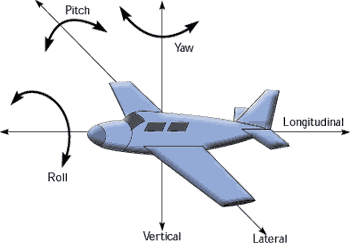
\includegraphics[width=5cm]{images/plane.png}
\end{center}

A rotation of the angle $\theta$ around the $X$-axes can be written as
\begin{equation}
R_X(\theta) \equiv \left(\begin{tabular}{ccc}
1 & 0 & 0 \\
0 & $\cos(\theta)$ & $-\sin(\theta)$  \\
0 & $\sin(\theta)$ & $\cos(\theta) $ 
\end{tabular}\right)
\end{equation}

A rotation of the angle $\theta$ around the $Y$-axes can be written as
\begin{equation}
R_Y(\theta) \equiv \left(\begin{tabular}{ccc}
$\cos(\theta)$ & 0 & $\sin(\theta)$ \\
0 & 1 & 0 \\
$-\sin(\theta)$ & 0 & $\cos(\theta)$ 
\end{tabular}\right)
\end{equation}

A rotation of the angle $\theta$ around the $Z$-axes can be written as
\begin{equation}
R_Z(\theta) = \left(\begin{tabular}{ccc}
$\cos(\theta)$ & $-\sin(\theta)$ & 0 \\
$\sin(\theta)$ & $\cos(\theta)$ & 0 \\
0 & 0 & 1
\end{tabular}\right)
\end{equation}

A rotation of the angle $\theta$ around an arbitrary direction $\hat n = (n_x,n_y,n_z)$ is given by:

\begin{equation}
R_{\hat n}(\theta) \equiv \left(\begin{tabular}{ccc} 
$t n_x n_x+c$ & $t n_x n_y-s n_z$ & $t n_x n_z+s n_y$ \\
$t n_x n_y+s n_z$ & $t n_y n_y+c$ & $t n_y n_z-s n_x$ \\
$t n_x n_z-s n_y$ & $t n_y n_z+s n_x$ & $t n_z n_z+c$
\end{tabular}\right)
\end{equation}
where $c=\cos(\theta)$ and $s=\sin(\theta)$ and $t=(1-\cos(\theta))$.

\begin{center}
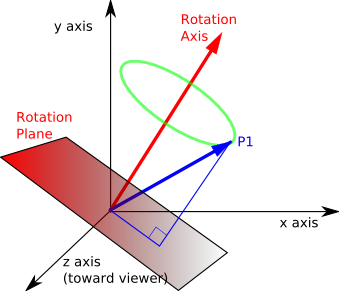
\includegraphics[width=5cm]{images/rotation.png}
\end{center}

\section{Composition of Rotations}

If a body is oriented according to $R_{\hat n}(\theta)$ and it gets rotated by another matrix $R_{\hat m}(\beta)$ the body will end up being oriented in a different direction:
\begin{equation}
R_{\hat n'}(\theta') = R_{\hat m}(\beta) R_{\hat n}(\theta)
\end{equation}
which we can rewrite with with a change of notation as
\begin{equation}
R' = R(\vec \beta) R
\end{equation}
where $R = R_{\hat n}(\theta)$, $R'=R_{\hat n'}(\theta')$, $R(\vec \beta)\equiv R_{\hat m}(\beta)$ and
\begin{equation}
\vec \beta = (\beta m_x, \beta m_y, \beta m_z)
\end{equation}
For an infinitesimal rotation $\beta = \omega dt$ we can write
\begin{equation}
R' = R(\vec \omega dt) R
\end{equation}
where
\begin{equation}
\vec \omega \equiv (\omega n_x, \omega n_y, \omega n_z)
\label{avelocity}
\end{equation}
is called angular velocity.

\section{Spinning Objects}

When a body is rotating with contant angular velocity $\vec \omega$, its rotation is proportional to time $t$ only. We say the body is spinning. Here we consider body spinning around the direction $\hat n=(n_x,n_y,n_z)$ of an anglular velocity $\omega$. The angular position of the object at time $t$ is therefore $\theta_t = \omega t$.
It is orinetation at time $t$ is therefore given by:
\begin{equation}
\vec \theta_t \equiv (\omega t n_x, \omega t n_y, \omega t n_z)
\end{equation}
So if we now consider the position of a vector $\vec p$ subject to rotation we obtain:
\begin{equation}
\vec p_t = R(\vec \theta_t) \vec p
\label{rottheta}
\end{equation}
and we can compute it velocity using the definition:
\begin{eqnarray}
\vec v_t &=& (\vec p_{t+dt} - \vec p_t)/dt \\
         &=& (R(\vec \theta_{t+dt}t) \vec p - R(\vec \theta_t) \vec p)/dt \\
         &=& \vec \omega \times \vec p
\label{vomega}
\end{eqnarray}
where $\vec \omega$ is the angular velocity, same as eq.~\ref{avelocity}.

\section{Newton Second Law for Rotation}

Before we have formulated the second law of Newton as
\begin{equation}
\vec F_t = \frac{\vec K_{t+dt}-\vec K_t}{dt}
\end{equation}
where $\vec K_t = m_t \vec v_t$.
We now consider a rigid body comprised of one mass $m$ at position $\vec p$, connected by a solid rod at the origin of the axes. The mass is subject to a force $\vec F$.

If there were no rod, the mass would move according to the Newton equation above. Because of the rod, the mass is not free and it feels only the component of the force ortoghonal to the direction of the rod $\vec r$ which is the same as the position of the mass $\vec p$ because the rod is pinned at the origin of the axes. In order to apply Newton law only to the components orthogonal to $r$ we perform a cross product of both terms

\begin{eqnarray}
\vec r_t \times \vec F_t &=& \vec r_t \times \frac{\vec  K_{t+dt}-\vec  K_t}{dt} \\
&=&  \frac{\vec r_t \times\vec K_{t+dt}-\vec r_t \times \vec  K_t}{dt}
\label{angular}
\end{eqnarray}
and if we define the {\it torque} as
\begin{equation}
\vec \tau \equiv \vec r \times \vec F
\end{equation}
and the {\it angular momentum} as
\begin{equation}
\vec L \equiv \vec r \times \vec K = m  \vec r \times \vec v
\label{angular_momentum}
\end{equation}
we can rewrite eq.~\ref{angular} as 
\begin{equation}
\vec \tau_ t = \frac{L_{t+dt}-L_t}{dt}
\label{newton_rot}
\end{equation}
which is the anologous of {\it Newton equation for rotations}.

\begin{center}
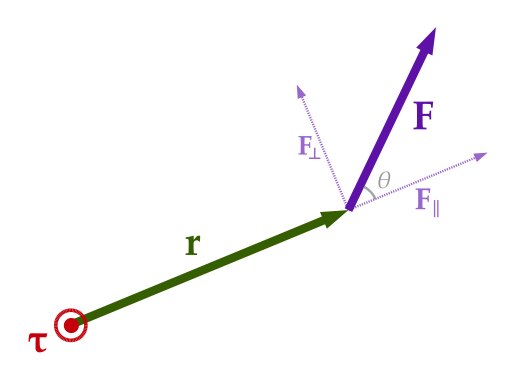
\includegraphics[width=5cm]{images/torque.png}
\end{center}

Notice that if we substiture eq.~\ref{vomega} which gives the velocity in terms of the angualar velocity into eq.~\ref{angular_momentum} we obtain:
\begin{equation}
\vec L = \vec r \times (m \vec \omega \times \vec r) = (m |\vec r|^2) \vec \omega
\label{angular_momentum2}
\end{equation}
The coefficient $(m |\vec r|^2)$ is called {\it moment of inertia}.

For a rigid body comprised of many masses rotating at the origin of the axes we can define:
\begin{equation}
\vec \tau \equiv \sum_i \vec r_i \times \vec F_i
\end{equation}
and
\begin{equation}
\vec L \equiv \sum_i \vec r_i \times \vec K_i = m_i  \vec r_i \times \vec v_i
\label{angular_momentum3}
\end{equation}
and eq.~\ref{newton_rot} is still valid, while eq.~\ref{angular_momentum3} becomes:
\begin{equation}
\vec L = \sum _i \vec r_i \times (m_i \vec \omega \times \vec r_i) = I \vec \omega
\label{angular_momentum4}
\end{equation}
where $I$ is a 3x3 matrix, called {\it Inertia Tensor} with components:
\begin{equation}
I_{jk} \equiv \sum_i m_i (\delta_{jk} |\vec r_i|^2 - r_{i,j} r_{i,k})
\label{momentum_inertia}
\end{equation}
Here $r_{i,j}$ is the $j$-th component (X=0,Y=1, or Z=2) of vector $\vec r_i$.


Finally we can augment the Euler integrator with equivelent formulas for rotations:
\begin{eqnarray}
\vec F_t =& \sum_i \vec F_i & \qquad \textrm{(compute force)} \\
\vec \tau_t =& \sum_i \vec r_i \times \vec F_i & \qquad \textrm{(compute torque)}\\
\vec v_{t} =& m_t^{-1}\vec K_{t} & \qquad \textrm{(compute velocity)}\\
\vec \omega_t =& I_t^{-1} L_t & \qquad \textrm{(compute angular velocity)}\\
\vec p_{t+dt} =& \vec p_t + \vec v_t dt & \qquad \textrm{(update position)}\\
\vec K_{t+dt} =& \vec K_t + \vec F_t dt & \qquad \textrm{(update momentum)}\\
% \tilde \theta_{t+dt} =& \tilde \theta_t + \frac{1}{2} \vec \omega_t \tilde \theta_t dt &  \qquad \textrm{(update orientation)}\\
R_t = & R(\omega_t dt) R_t & \qquad \textrm{(update orientation)}\\
\vec L_{t+dt} =& \vec L_t + \vec \tau_t dt & \qquad \textrm{(update angular momentum)}
\label{euler22}
\end{eqnarray}

In other words: {\it If we know the state of the rigid body characterized by the position $p_t$ and momentum $K_t$ of its center of mass, if we know its orientation $T_t$ and its angular momentum $L_t$, and if we know the total force $F_t$ and the total torque $\tau_t$ acting on the body, we can compute new state of the rigid body ($p,K,R,L$) at time $t+dt$.}

Given the position $p_t$ of the center of mass of the body and its orientation $\tilde \theta_t$, a generic point $\vec r_i$ of the body, can be rotated and translated into the global reference frame according to:
\begin{equation}
R_t \vec r_i + p_t
\end{equation}
and the velocity of the point is
\begin{equation}
\vec \omega_t \times \vec r_i + \vec v_t
\end{equation}

%($R(...)$ is described in eq.~\ref{rotation}).

\section{Quaternions}

Quaterions provide a way to representant an orientation in 3D without using a rotation but using a 4-vector instead. They are not used in the code because they are not necessary.

It can be convenient to define a four dimension vector (marked by a tilde):
\begin{equation}
\tilde \theta = (\theta_0,\theta_1,\theta_2,\theta_3) = (n_x \sin(\theta/2), n_y \sin(\theta/2), n_z \sin(\theta/2),\cos(\theta/2))
\label{quaternion}
\end{equation}
and with a change of variable the matrix of rotation $R_{\hat n}(\theta)$ can be re-written:

\begin{equation}
R(\tilde \theta) \equiv \left(\begin{tabular}{ccc}
$2(\theta_0 \theta_0 + \theta_1 \theta_1)-1$ & $2(\theta_0 \theta_1 - \theta_2 \theta_3)$ & $2(\theta_0 \theta_2 - \theta_1 \theta_3) $\\
$2(\theta_0 \theta_1 + \theta_2 \theta_3)$ & $2(\theta_1 \theta_1 +\theta_3 \theta_3)-1$ & $2(\theta_1 \theta_2-\theta_0 \theta_3) $\\
$2(\theta_0 \theta_3 - \theta_1 \theta_3)$ & $2(\theta_0 \theta_3 + \theta_1 \theta_2)$ & $2(\theta_2 \theta_2 + \theta_3 \theta_3)-1$
\end{tabular}\right)
\label{rotation}
\end{equation}

The 4-vector $\tilde \theta$ defines an {\it orientation} and it is called a {\it quaternion} although its mathematical properties are not relevant here and are not discussed. The associated matrix $R(\tilde \theta)$ can be used to rotates the points of an object into an orientation.

If a body is oriented according to $R(\tilde \theta)$ and it gets rotated by another matrix $R_{\hat n}(\beta)$ the body will end up being oriented in a different direction:
\begin{equation}
R(\tilde \theta') = R_{\hat n}(\beta) R(\tilde \theta)
\end{equation}

What's  $\tilde \theta'$ as function of $\hat n$, $\beta$ and $\tilde \theta$?
An explicit calculation (omitted) reveals:
\begin{equation}
\tilde \theta' = \tilde \theta + \frac{1}{2}\vec \beta \tilde \theta
\label{theta_update}
\end{equation}
where $\vec \beta \tilde \theta$ is defined as 
\begin{equation}
\vec \beta \tilde \theta = \left(\begin{tabular}{c}
$- (\beta_0 \theta_0 + \beta_1 \theta_1 + \beta_2 \theta_2)$ \\
$(\beta_0 \theta_3 + \beta_1 \theta_2 - \beta_2 \theta_1)$ \\ 
$(\beta_1 \theta_3 + \beta_2 \theta_0 - \beta_0 \theta_2)$ \\ 
$(\beta_2 \theta_3 + \beta_0 \theta_1 - \beta_1 \theta_0)$ 
\label{vxq}
\end{tabular}\right)
\end{equation}

where $(\beta_0,\beta_1,\beta_2)=(\beta n_x,\beta n_y,\beta n_z)$

Eq.~\ref{theta_update} will come up handy later when talking about spinning objects. In this case for an infinitesimal rotation $\beta=\omega dt$:
\begin{equation}
\tilde \theta' = \tilde \theta + \frac{1}{2}\vec \omega \tilde \theta dt
\end{equation}

\section{Assembling Rigid Bodies}

Consider a composite rigid body whose parts are smaller rigid bodies characterized by
\begin{center}
\begin{tabular}{cccc} \hline
Component & Position & Mass & Moment of Inertial \\ \hline
0 & $\vec p_0$ & $m_0$ & $I_0$ \\ 
1 & $\vec p_1$ & $m_1$ & $I_1$ \\ 
2 & $\vec p_2$ & $m_2$ & $I_2$ \\ 
... & ... & ... & ... \\ \hline
\end{tabular}
\end{center}

The composite object will have:
\begin{eqnarray}
m_{total} &=& \sum_i m_i \\
\vec p_{cm} &=& \sum \vec p_i m_i/m_{total} \\
I_{total} &=& \sum_i I_i + \Delta I(m_i, \vec p_i - \vec p_{total})
\end{eqnarray}
where
\begin{equation}
\Delta I(m, \vec r)_{jk} \equiv m (\delta_{jk} |\vec r|^2 - r_j r_k)
\end{equation}

The object $I$ is a $3\times 3$ matrix and it is called {\it Inertia Tensor}. The inertia tensor depends on the orienttation of the object. If the object is rotated by $R$, the inertia tensor changes as:

\begin{equation}
I \rightarrow I' = R I R^{-1}
\end{equation}

\section{Collisions}

Let's first consider particles instead of rigid bodies.

Given the velocities of two bodies $\vec v_A$ and $\vec v_B$ before a collision we want to determine the velocities of the bodies after the collision, $\vec v'_A$ and $\vec v'_B$. The separating velocity (relative velocity after the collision) is defined as:
\begin{equation}
\vec v_{separating} \equiv \vec v'_B - \vec v'_A
\end{equation}
If it is a faction of the closing velocity (relative velocity before the collision):
\begin{equation}
\vec v_{separating} = -c \vec v_{closing}
\label{collision}
\end{equation}
where $c$ is a restitution coefficient and 
\begin{equation}
\vec v_{closing} \equiv \vec v_B - \vec v_A
\end{equation}
Conservation of momentum and the above relation between closing and separating velocity yields:
\begin{eqnarray}
\vec K'_A &=& \vec K_A + \vec J/{m_A} \\
\vec K'_B &=& \vec K_B - \vec J/{m_B} 
\end{eqnarray}
where
\begin{equation}
\vec J = \frac{(c+1)(\vec v_B-\vec v_A)}{1/m_A+1/m_B}
\end{equation}

In the case of collision of the object A with a plane B or other object of infinite mass
\begin{equation}
\vec K'_A = \lim_{m_A-\rightarrow \infty} \vec K_A + \frac{\vec J}{m_A} = \vec K_A + m_A (c+1)(\vec v_B-\vec v_A)
\end{equation}

In the case of rigid bodies eq.~\ref{collision} applies to the points of contact between two rigid bodies. To properly consider its effect on the entire body we have to rewrite the velocity in terms of the velocities of the center of mass plus a component due to the angular velocity.

\begin{equation}
{\vec J}_{\perp} = \frac {-(c+1) (\vec v_{cB} - \vec v_{cA}) \cdot \hat n}{1/m_A+1/m_B + \left[ (1/I_A)(\vec r_{cA} \times \hat n)\times r_{cA}  + (1/I_B)(\vec r_{cB} \times \hat n) \times r_{rB}\right] \cdot {\hat n}}{\hat n}
\label{impulse}
\end{equation}

where $\vec r_{cA}$ is the point of collision of body A respect to the center of mass $\vec p_A$, $\vec v_{cA}$ is the velocity of the collision point before the collision, $m_A$ is the mass of body A, $I_A$ is its moment of inertia. $\hat n$ is a versor orthogonal to the contact point. Notice that $\vec r_{cA} = R_A\vec r_A$ and $\vec v_{cA} = \vec \omega_A \times \vec r_A + \vec v_A$. The same for $B$.

Once this impulse is computed we can deal with the it for each body by adding the contribution of the impulse to force and torque.

In presence of friction at the contact point, there is also a tangential impulse to take into account:

\begin{equation}
{\vec J}_{\parallel} = \frac{-(c_f+1) (\vec v_{cB} - \vec v_{cA}) \cdot \hat t}{1/m_A+1/m_B + \left[ (1/I_A)(\vec r_{cA} \times \hat t)\times r_{cA}  + (1/I_B)(\vec r_{cB} \times \hat t) \times r_{rB}\right] \cdot {\hat t}}{\hat t}
\label{impulse}
\end{equation}

where $\hat t$ is a versor orthogonal to $n$ and to the relative velocity beween the colliding points. In general $c_f$ is different from $c$.

\begin{eqnarray}
\vec K'_A &=& K_A + (\vec J_{\perp}+\vec J_{\parallel}) \\
\vec \tau'_A &=& \tau_A + \vec r_{cA} \times (\vec J_{\perp}+\vec J_{\parallel}) \\
\vec K'_B &=& K_B - (\vec J_{\perp}+\vec J_{\parallel}) \\
\vec \tau'_B &=& \tau_B - \vec r_{cB} \times (\vec J_{\perp}+\vec J_{\parallel}) 
\label{impulse2}
\end{eqnarray}

For if two objects we do the following:
\begin{itemize}
\item find the point of contact and compute $r_{cA}$, $r_{cB}$
\item find the compenetration and shift the objects back to cancel compenetration
\item compute the impulse (eq.~\ref{impulse})
\item update the force and torque to include one time contribution of the impulse (eq.~\ref{impulse2}).
\end{itemize}

\section{Geometry of collision}

Here we are concerned with the problem of terminating if two objects have collided. If the objects are made of vertices and faces the possible collisions can be vertex-vertex, vertex-edge, verted-face, edge-face, face-face. Most of them can be ignored but vertex-face and edge-edge.

Let's focus on vertex-face collision. In order to resolve the collisions we need to:
\begin{itemize}
\item detect a collision has occurred
\item find the normal to the collision
\item find the collision point
\item find the penetration
\end{itemize}

(not necessarily in this order). We will assume the body is convex (the center of mass is inside the body).

We will label $\vec p_A$ the center of mass of body $A$, $\vec p_B$ the center of mass of body $B$, $\vec q$ the collision point, $\hat n$ the normal to the collision point, $\vec f_1$,$\vec f_2$,$\vec f_3$ the vertices of the face of $A$ and $\vec u$ the vertex of body $B$ which may have hit the face of object $A$.

First we compute $\vec n$:
\begin{equation}
\vec n = (\vec f_2 - \vec f_1) \times (\vec f_3 - \vec f_1)
\end{equation}
and normalized it $\hat n = \vec n / n$.
Than we compute $q$:
\begin{equation}
\vec q = \vec u - (\vec u \cdot \hat n - \vec f_1 \cdot \hat n){\hat n}
\end{equation}
And we check that $\vec q$ lays inside the face:
\begin{eqnarray}
|(\vec q - \vec f_1)\times(\vec f_2-\vec f_1)|&+& \\
|(\vec q - \vec f_2)\times(\vec f_3-\vec f_2)|&+& \\
|(\vec q - \vec f_3)\times(\vec f_1-\vec f_3)| &<=& |(\vec f_1 - \vec f_2)\times(\vec f_3-\vec f_1)|
\end{eqnarray}
If this is the case, we check the the projection along $\hat n$ of the points $\hat p_A$ (the center of mass of $A$), the vertex $\hat v$, the collision point $\vec q$ and $\vec p_B$ (the center of mass of $B$) and in proper spatial order:
\begin{equation}
((\vec p_A - \vec p_B) \cdot \hat n) ((\vec u - \vec q) \cdot\hat n) >=0
\end{equation}
If the collision occurs the penetration is $\vec p - \vec q$.

Finally we loop over all faces of $A$, and vertices of $B$, we run the above algorithm and if a collision occurs we resolve the penetration, we compute the velocity of the collision point and we apply the impulse at collision point as discussed in the previous section.

\section{Implementation}


Import the necessary libraries
\begin{lstlisting}
#include "fstream"
#include <sstream>
#include <string>
#include <iostream>

#include "math.h"
#include "vector"
#include "set"

#if defined(_MSC_VER)
#include <gl/glut.h>
#else
#include <GLUT/glut.h>
#endif

using namespace std;
\end{lstlisting}

Define macros and constants
\begin{lstlisting}
#define array vector // to avoid name collions
#define forXYZ(i) for(int i=0; i<3; i++)
const float PRECISION = 0.00001;
const int X=0;
const int Y=1;
const int Z=2;
const int W=3; // for quaternions only
const float gravity = 9.8; // meters/second^2
\end{lstlisting}

Define class Vector
\begin{lstlisting}
class Vector {
public:
  float v[3];
  Vector(float x=0, float y=0, float z=0) {
    v[X]=x; v[Y]=y; v[Z]=z;
  }
  float operator()(int i) const { return v[i]; }
  float &operator()(int i) { return v[i]; }
};
\end{lstlisting}

Define operations between vectors
\begin{lstlisting}
Vector operator*(float c, const Vector &v) {
  return Vector(c*v(X),c*v(Y),c*v(Z));
}
Vector operator*(const Vector &v, float c) {
  return c*v;
}
Vector operator/(const Vector &v, float c) {
  return (1.0/c)*v;
}
Vector operator+(const Vector &v, const Vector &w) {
  return Vector(v(X)+w(X),v(Y)+w(Y),v(Z)+w(Z));
}
Vector operator-(const Vector &v, const Vector &w) {
  return Vector(v(X)-w(X),v(Y)-w(Y),v(Z)-w(Z));
}
float operator*(const Vector &v, const Vector &w) {
  return v(X)*w(X) + v(Y)*w(Y) + v(Z)*w(Z);
}
float norm(const Vector &v) {
  return sqrt(v*v);
}
Vector versor(const Vector &v) {
  float d=norm(v);
  return (d>0)?(v/d):v;
}
Vector cross(const Vector &v, const Vector &w) {
  return Vector(v(Y)*w(Z)-v(Z)*w(Y),
		v(Z)*w(X)-v(X)*w(Z),
		v(X)*w(Y)-v(Y)*w(X));
}
\end{lstlisting}

Class Rotation
\begin{lstlisting}
class Matrix {
public:
  float m[3][3];
  Matrix() { forXYZ(i) forXYZ(j) m[i][j]=0; }
  const float operator()(int i, int j) const { return m[i][j]; }
  float &operator()(int i, int j) { return m[i][j]; }
};

class Rotation : public Matrix {
public:
  Rotation() { forXYZ(i) forXYZ(j) m[i][j]=(i==j)?1:0; }
  Rotation(const Vector& v) {
    float theta = norm(v);    
    if(theta<PRECISION) {
      forXYZ(i) forXYZ(j) m[i][j] = (i==j)?1:0;
    } else {
      float s = sin(theta), c=cos(theta);
      float t = 1-c;
      float x = v(X)/theta, y = v(Y)/theta, z = v(Z)/theta;
      m[X][X]=t*x*x+c;   m[X][Y]=t*x*y-s*z; m[X][Z]=t*x*z+s*y;
      m[Y][X]=t*x*y+s*z; m[Y][Y]=t*y*y+c;   m[Y][Z]=t*y*z-s*x;
      m[Z][X]=t*x*z-s*y; m[Z][Y]=t*y*z+s*x; m[Z][Z]=t*z*z+c;
    }
  }
};
\end{lstlisting}

Class Inertia Tensor
\begin{lstlisting}
class InertiaTensor : public Matrix {};
InertiaTensor operator+(const InertiaTensor &a, const InertiaTensor &b) {
  InertiaTensor c=a;
  forXYZ(i) forXYZ(j) c(i,j)+=b(i,j);
  return c;
}
\end{lstlisting}

Operations between matrices
\begin{lstlisting}
Vector operator*(const Matrix &R, const Vector &v) {
  return Vector(R(X,X)*v(X)+R(X,Y)*v(Y)+R(X,Z)*v(Z),
		 R(Y,X)*v(X)+R(Y,Y)*v(Y)+R(Y,Z)*v(Z),
		 R(Z,X)*v(X)+R(Z,Y)*v(Y)+R(Z,Z)*v(Z));
}
Matrix operator*(const Matrix &R, const Matrix &S) {
  Matrix T;
  forXYZ(i) forXYZ(j) forXYZ(k) T(i,j)+=R(i,k)*S(k,j);
  return T;
}
float det(const Matrix &R) {
  return R(X,X)*(R(Z,Z)*R(Y,Y)-R(Z,Y)*R(Y,Z))
    -R(Y,X)*(R(Z,Z)*R(X,Y)-R(Z,Y)*R(X,Z))
    +R(Z,X)*(R(Y,Z)*R(X,Y)-R(Y,Y)*R(X,Z));
}
Matrix operator/(float c, const Matrix &R) {
  Matrix T;
  float d = c/det(R);
  T(X,X)=(R(Z,Z)*R(Y,Y)-R(Z,Y)*R(Y,Z))*d;
  T(X,Y)=(R(Z,Y)*R(X,Z)-R(Z,Z)*R(X,Y))*d;
  T(X,Z)=(R(Y,Z)*R(X,Y)-R(Y,Y)*R(X,Z))*d;
  T(Y,X)=(R(Z,X)*R(Y,Z)-R(Z,Z)*R(Y,X))*d;
  T(Y,Y)=(R(Z,Z)*R(X,X)-R(Z,X)*R(X,Z))*d;
  T(Y,Z)=(R(Y,X)*R(X,Z)-R(Y,Z)*R(X,X))*d;
  T(Z,X)=(R(Z,Y)*R(Y,X)-R(Z,X)*R(Y,Y))*d;
  T(Z,Y)=(R(Z,Y)*R(X,Y)-R(Z,Y)*R(X,X))*d;
  T(Z,Z)=(R(Y,Y)*R(X,X)-R(Y,X)*R(X,Y))*d;
  return T;
}
\end{lstlisting}

Class Body (describes a rigid body object)
\begin{lstlisting}
class Body {
public:
  // object shape
  float radius;     // all vertices inside radius;
  array<Vector> r;  // vertices in local coordinates
  array<array<int> > faces;
  // properties of the body /////////////////////////
  bool locked;       // if set true, don't integrate
  float m;           // mass
  InertiaTensor I;   // moments of inertia (3x3 matrix)
  // state of the body //////////////////////////////
  Vector p;          // position of the center of mass
  Vector K;          // momentum
  Matrix R;          // orientation
  Vector L;          // angular momentum
  // auxiliary variables ///////////////////////////
  float inv_m;       // 1/m
  Matrix inv_I;      // 1/I
  Vector F;
  Vector tau;
  Vector v;          // velocity
  Vector omega;      // angular velocity
  array<Vector> Rr; // rotated r's.
  array<Vector> vertices; // rotated and shifted r's
  // forces and constraints
  // ...
  Body(float m=1.0, bool locked=false) {
    radius = 0;
    this->locked = locked;
    this->m = 1.0;
    I(X,X)=I(Y,Y)=I(Z,Z)=m;
    inv_m = 1.0/m;
    inv_I = 1.0/I;
    R = Rotation();
  };
  void clear() { F(X)=F(Y)=F(Z)=tau(X)=tau(Y)=tau(Z)=0; }
  void update_vertices();
  void integrator(float dt);
  void loadObj(const string & file);
};
\end{lstlisting}

rotate and shift all vertices from local to universe
\begin{lstlisting}
void Body::update_vertices() {
  Rr.resize(r.size());
  vertices.resize(r.size());
  for(int i=0; i<r.size(); i++) {
     Rr[i] = R*r[i];
     vertices[i]=Rr[i]+p;
  }
}
\end{lstlisting}

Euler integrator
\begin{lstlisting}
void Body::integrator(float dt) {
  v     = inv_m*K;
  omega = inv_I*L;
  p     = p + v*dt;                // shift
  K     = K + F*dt;                // push
  R     = Rotation(omega*dt)*R;    // rotate
  L     = L + tau*dt;              // spin
  update_vertices();
}
\end{lstlisting}

Interface for all forces.
The constructor can be specific of the force
the apply methods adds the contribution to F and tau
\begin{lstlisting}
class Force {
public:
  virtual void apply(float dt)=0;
};
\end{lstlisting}

Gravity
\begin{lstlisting}
class GravityForce : public Force {
public:  
  Body *body;
  float g;
  GravityForce(Body *body, float g = gravity) {
    this->body=body; this->g=g;    
  }
  void apply(float dt) {
    body->F(Y) -= (body->m)*g;
  }
};
\end{lstlisting}

Spring Forces
\begin{lstlisting}
class SpringForce : public Force {
public:
  Body *bodyA;
  Body *bodyB;
  int iA, iB;
  float kappa, L;
  SpringForce(Body *bodyA, int iA, Body *bodyB, int iB,
	      float kappa, float L) {
    this->bodyA=bodyA; this->iA=iA;
    this->bodyB=bodyB; this->iB=iB;
    this->kappa=kappa; this->L=L;
  }
  void apply(float dt) {
    Vector d = bodyB->vertices[iB]-bodyA->vertices[iA];
    float n = norm(d);
    if(n>PRECISION) {
      Vector F = kappa*(n-L)*(d/n);
      bodyA->F = bodyA->F+F;
      bodyB->F = bodyB->F-F;
      bodyA->tau = bodyA->tau + cross(bodyA->Rr[iA],F);
      bodyB->tau = bodyB->tau - cross(bodyB->Rr[iB],F);
    }
  }
};

class AnchoredSpringForce : public Force {
public:
  Body *body;
  int i;
  Vector pin;
  float kappa, L;
  AnchoredSpringForce(Body *body, int i, Vector pin,
		      float kappa, float L) {
    this->body=body; this->i=i;
    this->pin = pin;
    this->kappa=kappa; this->L=L;
  }
  void apply(float dt) {
    Vector d = body->vertices[i]-pin;
    float n = norm(d);
    Vector F = kappa*(n-L)*d/n;
    body->F = body->F+F;
    body->tau = body->tau + cross(body->Rr[i],F);
  }
};
\end{lstlisting}

Friction (ignores the shape of the body, assumes a sphere)
\begin{lstlisting}
class FrictionForce: public Force {
public:
  Body *body;
  float gamma;
    FrictionForce(Body *body, float gamma) {
      this->body=body; this->gamma=gamma;
    }
    void apply(float dt) {
      body->F = body->F-gamma*(body->v)*dt; // ignores shape
    }
};
\end{lstlisting}

Class to deal with constraints (must be able to detect and resolve)
\begin{lstlisting}
class Constraint {
public:  
  virtual bool detect()=0;
  virtual void resolve(float dt)=0;
  Vector impluse(const Body &A, const Body &B, 
		 Vector &r_A, Vector &r_B, Vector n, float c) {
    float IA; // FIX
    float IB; // FIX
    Vector r_cA = A.R*r_A;
    Vector r_cB = B.R*r_B;
    Vector v_cA = cross(A.omega,r_A)+A.v;
    Vector v_cB = cross(B.omega,r_B)+B.v;
    Vector crossA = cross(r_cA,n);
    Vector crossB = cross(r_cB,n);
    Vector dF = (-(c-1)/(A.inv_m+B.inv_m+
			 crossA*crossA/IA+
			 crossB*crossB/IB)*(v_cB-v_cB)*n)*n;
  }
};
\end{lstlisting}

Class to deal with collision with static plane
(ignore rotation)
\begin{lstlisting}
class PlaneConstraint: public Constraint {
public:
  Body *body;
  Vector n,d;
  float penetration, restitution;
  // d is the discance of the plane from origin
  // n is a versor orthogonal to plane 
  // (in opposite direction from collision)
  PlaneConstraint(Body *body, float restitution,
		  const Vector &d, const Vector &n) {
    this->body = body;
    this->n=n; this->d=d;
    this->restitution = restitution;
  }
  bool detect() {
    penetration = body->p*n-d*n + body->radius;
    return penetration>=0;
  }
  void resolve(float dt) {
    // move the object back is stuck on plane 
    body->p = body->p - penetration*n;
    float K_ortho = n*body->K;
    // optional, deal with friction 
    Vector L_ortho = -(body->radius)*cross(n,body->K-K_ortho);
    Vector L_hat = versor(L_ortho);
    body->L = (n*body->L)*n + L_ortho;
    // reverse momentum
    if(K_ortho>0)
      body->K = body->K - (restitution+1)*(K_ortho)*n;
  }
};
\end{lstlisting}

class that stores all bodies, forces and constraints
\begin{lstlisting}
class Universe {
public:
  set<Body*> bodies;
  set<Force*> forces;
  set<Constraint*> constraints;
  set<Body*>::iterator body;
  set<Force*>::iterator force;
  set<Constraint*>::iterator constraint;
  int frame;
  Universe() { frame=0; }
  // evolve universe
  void evolve(float dt) {    
    // clear forces and troques
    for(body=bodies.begin(); body!=bodies.end(); body++)
      (*body)->clear();
    // compute forces and torques
    for(force=forces.begin(); force!=forces.end(); force++)
      (*force)->apply(dt); // adds to F and tau
    // test: give it a kick
    callback();
    // integrate
    for(body=bodies.begin(); body!=bodies.end(); body++) 
      if(!(*body)->locked)
	(*body)->integrator(dt);
    // handle collisions (not quite right yet)
    for(constraint=constraints.begin();
	constraint!=constraints.end(); constraint++)
      if((*constraint)->detect())
	(*constraint)->resolve(dt);
    frame++;
  }
public:
  virtual void build_universe()=0;
  virtual void callback()=0;
};
\end{lstlisting}

Auxiliary functions translate moments of Inertia
\begin{lstlisting}
InertiaTensor dI(float m, const Vector &r) {
  InertiaTensor I;
  float r2 = r*r;
  forXYZ(j) forXYZ(k) I(j,k) = m*((j==k)?r2:0-r(j)*r(k));
  return I;
}
\end{lstlisting}

Auxliary function to include to merge two bodies
needs some more work....
\begin{lstlisting}
Body operator+(const Body &a, const Body &b) {
  Body c;
  c.m = (a.m+b.m);
  c.p = (a.m*a.p + b.m+b.p)/c.m;
  c.K = a.K+b.K;
  c.L = (a.p-c.p)*a.K+(b.p-c.p)*b.K;
  Vector da = a.p-c.p;
  Vector db = b.p-c.p;
  c.I = a.I+dI(a.m,da)+b.I+dI(b.m,db);
  int n = a.r.size();
  // copy all r
  for(int i=0; i<n; i++)
    c.r.push_back(a.r[i]+da);
  for(int i=0; i<b.r.size(); i++)
    c.r.push_back(b.r[i]+db);
  // copy all faces and re-label r  
  int m = a.faces.size();
  c.faces.resize(a.faces.size()+b.faces.size());
  for(int j=0; j<a.faces.size(); j++)
    c.faces[j]=a.faces[j];
  for(int j=0; j<b.faces.size(); j++)
    for(int k=0; k<b.faces[j].size(); k++)
      c.faces[j+m].push_back(b.faces[j][k]+n);  
  c.update_vertices();
  return c;
}

void Body::loadObj(const string & file) {
  ifstream input;
  input.open(file.c_str());
  string line;
  if(input.is_open()) {
    while(input.good()) {
      std::getline(input, line);
      if(line.length()>0) {
	string initialVal;
	istringstream instream;
	instream.str(line);
	instream >> initialVal;
	if(initialVal=="v") {
	  float x,y,z;
	  instream >> x >> y >> z;
	  r.push_back(Vector(x,y,z));
	  radius = max(radius,norm(Vector(x,y,z)));
	} else if (initialVal=="f") {
	  int v1, v2, v3;
	  instream >> v1 >> v2 >> v3;
	  array<int> triangle;
	  triangle.push_back(v1-1);
	  triangle.push_back(v2-1);
	  triangle.push_back(v3-1);
	  faces.push_back(triangle);
	}
      }
    }
    update_vertices();
  }
}
\end{lstlisting}

GLUT code below
Creates a window in which to display the scene.
\begin{lstlisting}
void createWindow(const char* title) {
  int width = 640;
  int height = 480;
  glutInitDisplayMode(GLUT_DOUBLE | GLUT_RGB | GLUT_DEPTH);
  glutInitWindowSize(width,height);
  glutInitWindowPosition(0,0);
  glutCreateWindow(title);
  
  glClearColor(0.9f, 0.95f, 1.0f, 1.0f);
  glEnable(GL_DEPTH_TEST);
  glShadeModel(GL_SMOOTH);
  
  glMatrixMode(GL_PROJECTION);
  glLoadIdentity();
  gluPerspective(60.0, (double)width/(double)height, 1.0, 500.0);
  glMatrixMode(GL_MODELVIEW);
}
\end{lstlisting}

My Universe!
\begin{lstlisting}
class MyUniverse : public Universe {
public:
  void build_universe() {
    Body *b_old=0;
    for(int i=0; i<4; i++) {
      Body *b = new Body();
      b->loadObj("assets/sphere.obj");
      b->p = Vector(i,i+2,-i);
      b->K = Vector(0.1*i,0.01*i,0);
      b->L = Vector(0.5,0.5*i,0);
      bodies.insert(b);
      forces.insert(new GravityForce(b,0.01));
      constraints.insert(
	new PlaneConstraint(b,0.9,Vector(0,0,0),Vector(0,-1,0)));
      constraints.insert(
	new PlaneConstraint(b,0.9,Vector(4,0,0),Vector(1,0,0)));
      constraints.insert(
        new PlaneConstraint(b,0.9,Vector(-4,0,0),Vector(-1,0,0)));
      constraints.insert(
        new PlaneConstraint(b,0.9,Vector(0,0,0),Vector(0,0,1)));
      constraints.insert(
        new PlaneConstraint(b,0.9,Vector(0,0,-5),Vector(0,0,-1)));
      // forces.insert(new FrictionForce(b,0.5));
      if(i==2)
	forces.insert(new SpringForce(b_old,0,b,0,0.01,0));
      b_old = b;
    }
  }
  void callback() {
    // kick the ball
    if(frame==2500) {
      (*bodies.begin())->F=Vector(10,10,0);
      (*bodies.begin())->tau=Vector(0,0,2);
      }
  }
};

MyUniverse universe;
\end{lstlisting}

Called each frame to update the 3D scene. Delegates to
the application.
\begin{lstlisting}
void update() {
  // evolve world
  float timeStep = 0.016f;	// 60fps fixed rate.
  universe.evolve(timeStep);
  glutPostRedisplay();
}
\end{lstlisting}

Called each frame to display the 3D scene. Delegates to
the application.
\begin{lstlisting}
void display() {
  glClear(GL_COLOR_BUFFER_BIT | GL_DEPTH_BUFFER_BIT);
  glLoadIdentity();
  gluLookAt(0.0, 3.5, 8.0,  0.0, 3.5, 0.0,  0.0, 1.0, 0.0);
  glColor3f(0,0,0);
  
  // draw
  for(universe.body=universe.bodies.begin();
      universe.body!=universe.bodies.end();
      universe.body++) {
    glPushMatrix();
    Vector &pos = (*universe.body)->p;
    glTranslatef(pos.v[X], pos.v[Y], pos.v[Z]);
    glPolygonMode(GL_FRONT_AND_BACK,GL_LINE);
    for(int i=0; i<(*universe.body)->faces.size(); i++) {      
      glBegin(GL_POLYGON);
      for(int j=0; j<(*universe.body)->faces[i].size(); j++) {
	int k = (*universe.body)->faces[i][j]; 
	glVertex3fv((*universe.body)->vertices[k].v);
      }
      int k = (*universe.body)->faces[i][0]; 
      glVertex3fv((*universe.body)->vertices[k].v);
      glEnd();
    }
    glPopMatrix();
  }
  // update the displayed content
  glFlush();
  glutSwapBuffers();
}
\end{lstlisting}

Called when the display window changes size.
\begin{lstlisting}
void reshape(int width, int height) {
  glViewport(0, 0, width, height);
}
\end{lstlisting}

Called when a mouse button is pressed. Delegates to the
application.
\begin{lstlisting}
void mouse(int button, int state, int x, int y) { }
\end{lstlisting}

Called when a key is pressed.
\begin{lstlisting}
void keyboard(unsigned char key, int x, int y) {
  // Note we omit passing on the x and y: they are rarely needed.
  //Process keyboard
}
\end{lstlisting}

Called when the mouse is dragged.
\begin{lstlisting}
void motion(int x, int y) { }
\end{lstlisting}

The main entry point. We pass arguments onto GLUT.
\begin{lstlisting}
int main(int argc, char** argv) {
  // Set up GLUT and the timers
  glutInit(&argc, argv);
    // Create the application and its window
  createWindow("GPNS");
  // fill universe with stuff
  universe.build_universe();
  // Set up the appropriate handler functions
  glutReshapeFunc(reshape);
  glutKeyboardFunc(keyboard);
  glutDisplayFunc(display);
  glutIdleFunc(update);
  glutMouseFunc(mouse);
  glutMotionFunc(motion);  
  // Run the application
  glutMainLoop();  
  // Clean up the application
  return 0;
}
\end{lstlisting}


\end{document}
